% !TEX root = ../main.tex
\section{Observed flood: Sentinel-1}
\label{sec:flood}

Radar sees through typhoon clouds. For each typhoon, new open water is mapped on Google Earth Engine from the vertical-horizontal (VH) backscatter of Sentinel-1 in 100~m tiles near the track: the before image is the median of days $-30$ to $-3$ and the after image the darkest of days 0 to $+$\sOneAfterDays{}, \textbf{both from the same relative orbit}. A pixel is new flood when its VH backscatter drops by at least 3~dB and ends at most $-18$~dB; permanent water, slopes over 5\textdegree{} and specks under 8 pixels are removed \parencite[after][]{unspider}. The first version, an after-to-before ratio on decibel values with mixed orbits, recovered almost none of the EMS flood and was replaced.

Figure~\ref{fig:s1} maps the new-flood share per unit and Table~\ref{tab:s1} gives the people in new flood per storm. Table~\ref{tab:s1muni} repeats this per municipality; there $\rho$ is the Spearman correlation, over the municipalities the radar saw, between network access loss $A$ and the new-flood share. Access loss follows flood but not one-to-one: a municipality can be flooded and keep a dry road to a hospital.

\begin{figure}[htbp]
\centering
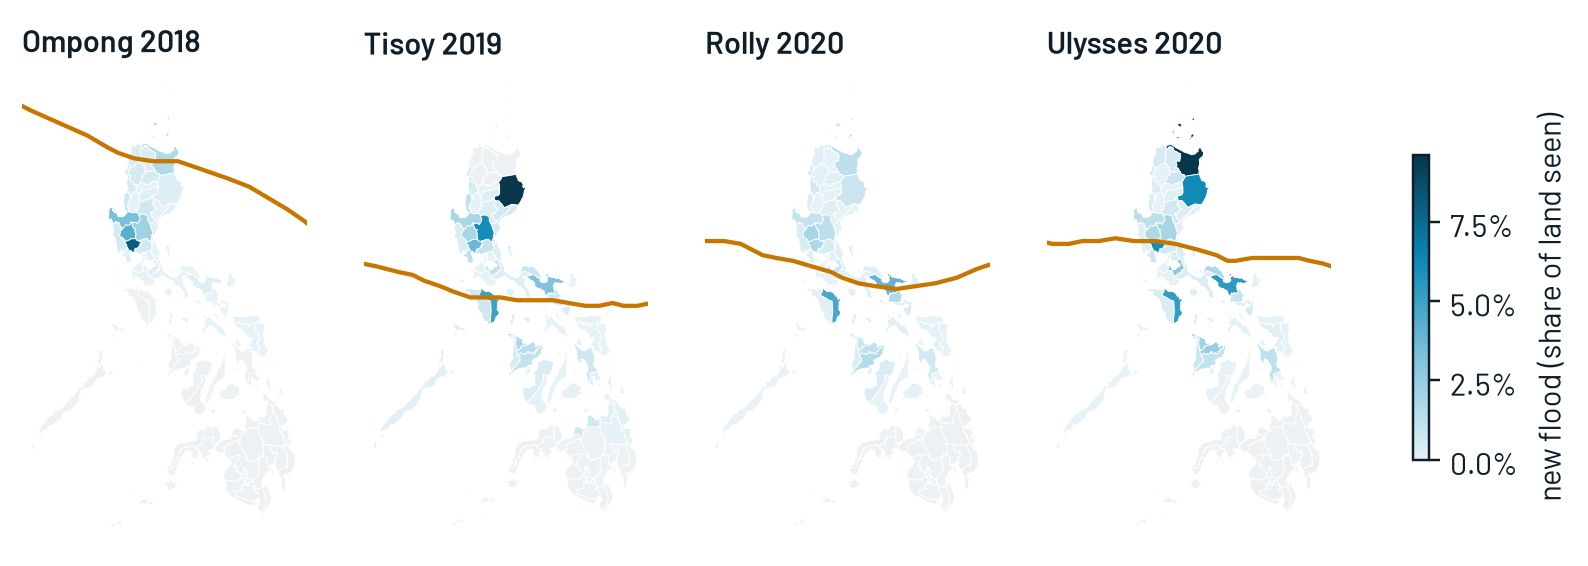
\includegraphics[width=\linewidth]{f11_s1_flood}
\caption{New-flood share of the land Sentinel-1 saw, per unit, with each typhoon's track.}
\label{fig:s1}
\end{figure}

\begin{table}[htbp]
\centering
\caption{People in new flood per typhoon, from the Sentinel-1 masks.}
\label{tab:s1}
\small
\begin{tabular}{@{}l r r r l@{}}
\toprule
typhoon & people in new flood & units $>$\sOneFloodThr{} flooded & max unit share & most people flooded \\
\midrule
\tablerows{s1}
\bottomrule
\end{tabular}
\end{table}

\begin{table}[htbp]
\centering
\caption{Sentinel-1 per municipality: municipalities seen over more than a fifth of their area, municipalities with more than \sOneFloodThr{} new flood, the three with most people in new flood, and the rank correlation of access loss with flood.}
\label{tab:s1muni}
\footnotesize
\begin{tabularx}{\linewidth}{@{}l r r L r@{}}
\toprule
typhoon & seen & flooded & most people in new flood: municipality (province), people, share & $\rho(A, \text{flood})$ \\
\midrule
\tablerows{s1muni}
\bottomrule
\end{tabularx}
\end{table}

\subsection{Checked against Copernicus EMS}

Inside the EMS areas of interest for Ompong, EMS mapped \emsKm{}~km\textsuperscript{2} of observed flood and Sentinel-1 flagged \sOneKm{}~km\textsuperscript{2}; \bothKm{}~km\textsuperscript{2} overlap. \textbf{\emsPrecision{}} of the Sentinel-1 flood there is confirmed by EMS, and Sentinel-1 recovers \textbf{\emsRecall{}} of the EMS area (Figure~\ref{fig:s1ems}).\ifEMSRecallLow{} Low recall is expected: EMS used other imagery and dates, while one Sentinel-1 orbit passed here only twice in the window.\fi

\begin{figure}[htbp]
\centering
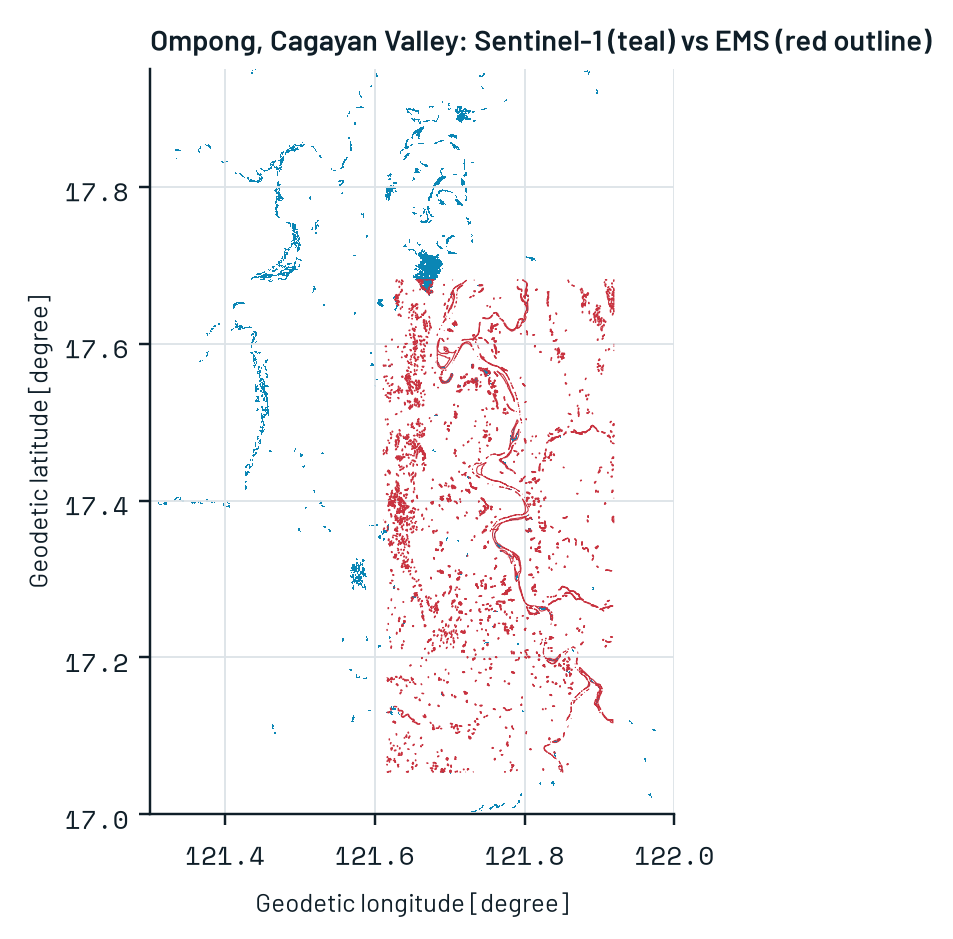
\includegraphics[width=0.55\linewidth]{f12_s1_ems}
\caption{Ompong around Tuguegarao: Sentinel-1 new flood (teal) and Copernicus EMS observed flood (red outlines).}
\label{fig:s1ems}
\end{figure}
